\documentclass[a4paper,12pt]{article}

\usepackage[14pt]{extsizes}
\usepackage{cmap}					% поиск в PDF
\usepackage{mathtext} 				% русские буквы в формулах
\usepackage[T2A]{fontenc}			% кодировка
\usepackage[utf8]{inputenc}			% кодировка исходного текста
\usepackage[english,russian]{babel}	% локализация и переносы
\usepackage{graphicx}
\usepackage{geometry}
\usepackage{amsmath}
\usepackage{amssymb}
\usepackage[table]{xcolor}
\usepackage{multirow}


\geometry{verbose, a4paper, tmargin=2cm, bmargin=2cm, lmargin=3cm, rmargin=2cm}
\author{Vysotsky Maxim}
\title{Отчёт}
\date{2022}

\begin{document}
	\begin{titlepage}
		\begin{center}
			{Министерство науки и высшего образования Российской Федерации
				НОВОСИБИРСКИЙ НАЦИОНАЛЬНЫЙ ИССЛЕДОВАТЕЛЬСКИЙ
				ГОСУДАРСТВЕННЫЙ УНИВЕРСИТЕТ (НГУ)}
		\end{center}
		\begin{center}
			{Физический факультет}
		\end{center}
		\begin{center}
			{Кафедра общей физики}
		\end{center}
		
		
		\vspace{7cm}
		{
			\begin{center}
				{\bf Лабораторная работа №3.2}\\
				Измерения с помощью электронно-лучевого
осциллографа
			\end{center}
		}
		\vspace{2cm}
		\begin{flushright}
			{Руководитель:\\ Старший преподаватель, к.ф.-м.н. \\
				Яцких А. А.\\
				Работу выполнил:\\
				Высоцкий М. Ю.\\
				\vspace{0.2cm}
				гр. 24301}
		\end{flushright}
		\vspace{3cm}
		\begin{center}
			Новосибирск, 2024
		\end{center}
	\end{titlepage}


\section{Теоретическое введение.}
\textbf{Цель работы:} понять основные принципы действия осциллографов и научиться использовать их для наблюдения и измерения характеристик электрических сигналов. В данной работе используется электронно-лучевой осциллограф Instek GOS-620.

В электронно-лучевых осциллографах экраном является передняя
стенка электронно-лучевой трубки, покрытая с внутренней стороны люминофором. Электронный луч, создаваемый электронной пушкой и управляемый напряжениями, подаваемыми на две пары пластин – вертикальную Y и горизонтальную Х, – перемещается по люминесцентному покрытию ЛС, "вычерчивая" соответствующую кривую (например, фигуру Лиссажу). Важно иметь в виду, что перемещение луча происходит в реальном времени, т.е. в каждый момент текущего времени его мгновенное положение соответствует именно этому моменту.

В электронно-лучевых осциллографах экраном является передняя
стенка электронно-лучевой трубки (рис. 2), покрытая с внутренней
стороны люминофором. Электронный луч, создаваемый электрон-
ной пушкой и управляемый напряжениями, подаваемыми на две
пары пластин – вертикальную Y и горизонтальную Х, – перемеща-
ется по люминесцентному покрытию ЛС, "вычерчивая" соответст-
вующую кривую (например, фигуру Лиссажу). Важно иметь в виду,
что перемещение луча происходит в реальном времени, т.е. в каж-
дый момент текущего времени его мгновенное положение соответ-
ствует именно этому моменту.

\begin{figure}[h!]
	\begin{center}
		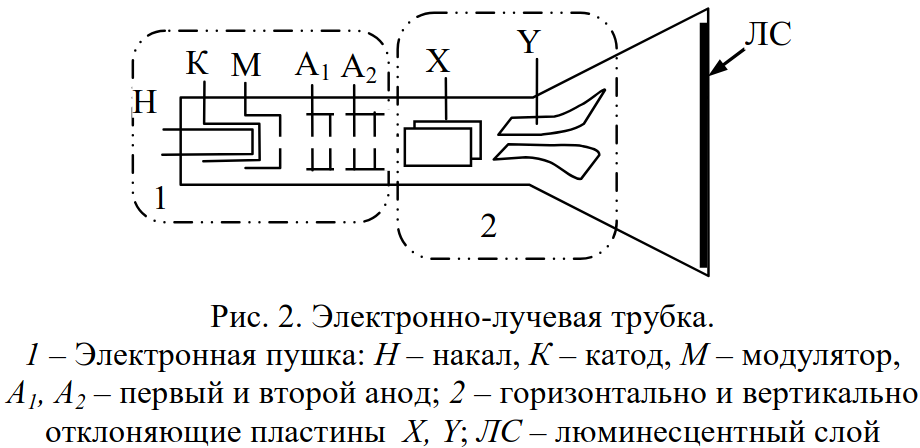
\includegraphics[scale=0.6]{ELT.png}
	\end{center}
	\caption{Устройство ЭЛТ.}
\end{figure}

\clearpage
\section{Ход работы}
\subsection{Задание 1. Освоение основных функций осциллографа.}
Потыкали, покрутили, похоже на правду. Калибратор тыкали (п.2), переключатели потыкали. Блок развёртки (п.3) и сихронизации (п.4) тоже потыкали.
\subsection{Задание 2. Знакомство с генераторами Г6-28 и GFG 8255.}
Потыкали, покрутили, познакомились с генераторами, они пожали нам руку.

\subsection{Задание 3. Исследование релаксационного генератора.}
\textbf{Цель задания:} научиться использовать осциллограф для исследования
сигналов с постоянной и переменной составляющей; измерить период колебаний релаксационного генератора на неоновой лампочке
и величину напряжение зажигания $U_з$ и гашения $U_г$ лампочки.

\begin{figure}[h!]
	\begin{center}
		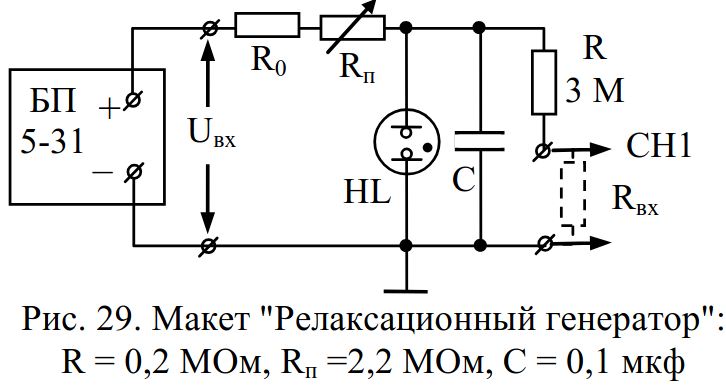
\includegraphics[scale=0.6]{scheme_3.png}
	\end{center}
	\caption{Макет "релаксационный генератор".}
\end{figure}

В (п.3) мы установили, что частота $\nu$ обратно сопротивлению $R_n$: $\nu \sim \frac{1}{R_n}$, а так же прямом пропорциональна выходному напряжению генератора $U$: $\nu \sim U$.

Это можно объяснить тем, что частота зависит от того, как быстро заряжается и разряжается конденсатор в цепи (по сути наша частота - это то, как часто конденсатор бывает разряжен в 0), а это обратно зависит от сопротивления и на прямую зависит от напряжения

Далее, мы установили на генераторе напряжение $U = 70В$. Это напряжение при максимальном сопротивлении, когда есть устойчивое изображение.

\begin{table}[!ht]
    \centering
    \begin{tabular}{|l|l|l|l|}
    \hline
        $U, В$ & $T, мс$ & $U_з$, В & $U_г, В$ \\ \hline
        70 & 3,5 & 10,8 & 6 \\ \hline
        80 & 2 & 10,8 & 3,4 \\ \hline
    \end{tabular}
    \caption{Данные задания 3.}
\end{table}

\subsection{Задание 4. Измерение времени распространения
сигнала в длинной линии.}
\textbf{Цель задания:} измерить время распространения сигнала по длинной линии; понять смысл включения согласующего переходника (согласованного сопротивления) при измерениях на высоких частотах.
\begin{figure}[h!]
	\begin{center}
		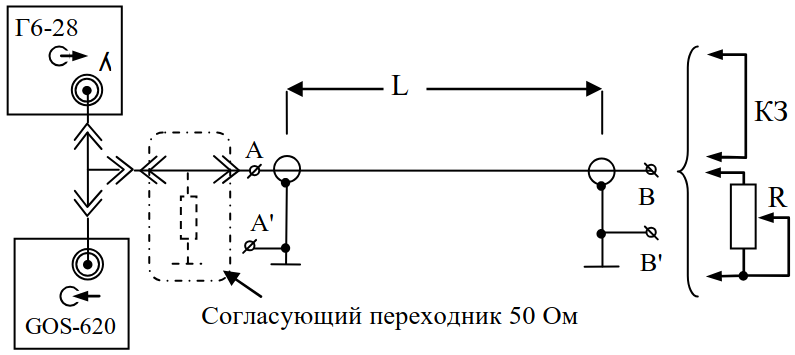
\includegraphics[scale=0.6]{scheme_4.png}
	\end{center}
	\caption{Макет "длинная линия".}
\end{figure}

Здесь была выставлена частота равная 0,49 МГц. Время между падающим и отраженным импульсом равно $t = 1$ мкс. А длина линии $L = 100$ м.
Далее нам дана формула:
\begin{equation}
    v = \frac{2L}{t}
\end{equation}
Таким образом, скорость распространения сигнала в линии $v = 2*10^8$ $\frac{М}{с}$


\end{document}

